%%%%%%%%%%%%%%%%%%%%%%%%%%%%%%%%%%%%%%%%%
% Beamer Presentation
% LaTeX Template
% Version 1.0 (10/11/12)
%
% This template has been downloaded from:
% http://www.LaTeXTemplates.com
%
% License:
% CC BY-NC-SA 3.0 (http://creativecommons.org/licenses/by-nc-sa/3.0/)
%
%%%%%%%%%%%%%%%%%%%%%%%%%%%%%%%%%%%%%%%%%

%------------------------------------------------------------------------------------------------
% PACKAGES AND THEMES
%------------------------------------------------------------------------------------------------

\documentclass[table, xcolor = {dvipsnames}, 9pt]{beamer}
\usepackage{tikz}
\usetikzlibrary{calc}
\usetikzlibrary{positioning}
\usetikzlibrary{arrows.meta}
\usetikzlibrary{external}
\mode<presentation> {

% The Beamer class comes with a number of default slide themes
% which change the colors and layouts of slides. Below this is a list
% of all the themes, uncomment each in turn to see what they look like.

\usetheme{default}
%\usetheme{AnnArbor}
%\usetheme{Antibes}
%\usetheme{Bergen}
%\usetheme{Berkeley}
%\usetheme{Berlin}
%\usetheme{Boadilla}
%\usetheme{CambridgeUS}
%\usetheme{Copenhagen}
%\usetheme{Darmstadt}
%\usetheme{Dresden}
%\usetheme{Frankfurt}
%\usetheme{Goettingen}
%\usetheme{Hannover}
%\usetheme{Ilmenau}
%\usetheme{JuanLesPins}
%\usetheme{Luebeck}
%\usetheme{Madrid}
\usetheme{metropolis}
%\usetheme{Malmoe}
%\usetheme{Marburg}
%\usetheme{Montpellier}
%\usetheme{PaloAlto}
%\usetheme{Pittsburgh}
%\usetheme{Rochester}
%\usetheme{Singapore}
%\usetheme{Szeged}
%\usetheme{Warsaw}

% As well as themes, the Beamer class has a number of color themes
% for any slide theme. Uncomment each of these in turn to see how it
% changes the colors of your current slide theme.

%\usecolortheme{albatross}
%\usecolortheme{beaver}
%\usecolortheme{beetle}
%\usecolortheme{crane}
%\usecolortheme{dolphin}
%\usecolortheme{dove}
%\usecolortheme{fly}
%\usecolortheme{lily}
%\usecolortheme{orchid}
%\usecolortheme{rose}
\usecolortheme{seagull}
%\usecolortheme{seahorse}
%\usecolortheme{whale}
%\usecolortheme{wolverine}
\usefonttheme{professionalfonts}
%\setbeamertemplate{footline} % To remove the footer line in all slides uncomment this line
%\setbeamertemplate{footline}[page number] % To replace the footer line in all slides with a simple slide count uncomment this line

%\setbeamertemplate{navigation symbols}{} % To remove the navigation symbols from the bottom of all slides uncomment this line
}

\usepackage{graphicx} % Allows including images
\usepackage{booktabs} % Allows the use of \toprule, \midrule and \bottomrule in tables
\usepackage{float}
\usepackage{tikz}
\usepackage{multirow}
\usepackage{natbib}
\usepackage{hyperref}
\usepackage{diagbox}
\usepackage{makecell}
\usepackage{xparse}
\usepackage{subfig}
\usepackage{amsmath}
\usepackage{amsfonts,amsthm,amsmath,amssymb}
\usepackage{bbm}
\usepackage{bm}
\usepackage{empheq}
\usepackage{pgfplots}
\usepackage{animate}
\usepgfplotslibrary{colorbrewer}
\pgfplotsset{compat=1.17}

\newcommand\mybox[2][]{\tikz[overlay]\node[fill=lightgray,inner sep=2pt, anchor=text, rectangle, rounded corners=1mm,#1] {#2};\phantom{#2}}
\hypersetup{unicode=true,
            bookmarksnumbered=true,
            bookmarksopen=true,
            bookmarksopenlevel=2,
            breaklinks=false,
            pdfborder={0 0 1},
            hypertexnames=false,
            pdfstartview={XYZ null null 1}}
\usepackage{xcolor}
% R code listing style (matches the course's R-code slides)
\usepackage{listings}
\definecolor{codegreen}{rgb}{0,0.6,0}
\definecolor{codegray}{rgb}{0.5,0.5,0.5}
\definecolor{codepurple}{rgb}{0.58,0,0.82}
\definecolor{backcolour}{rgb}{0.95,0.95,0.92}
\lstdefinestyle{Rstyle}{
    language=R,
    backgroundcolor=\color{backcolour},
    commentstyle=\color{codegreen},
    keywordstyle=\color{magenta},
    stringstyle=\color{codepurple},
    basicstyle=\ttfamily\footnotesize,
    breakatwhitespace=false,
    breaklines=true,
    keepspaces=true,
    showspaces=false,
    showstringspaces=false,
    showtabs=false,
    tabsize=2
}
\newcommand\myheading[1]{%
  \par\bigskip
  {\Large\bfseries#1}\par\smallskip}
\newcommand\given[1][]{\:#1\vert\:}
\theoremstyle{plain}
\newtheorem{thm}{Theorem}
\newtheorem{prop}{Proposition\thisthmnumber}
\newtheorem{lem}{Lemma\thisthmnumber}
\newtheorem{cor}{Corollary}
\newtheorem{defin}{Definition}
\newtheorem{algo}{Algorithm}
\newcommand*\diff{\mathop{}\!\mathrm{d}}
\newcommand*\Diff[1]{\mathop{}\!\mathrm{d^#1}}
\newcommand{\bh}[1]{{\color{blue}{#1}}}
\newcommand{\mh}[1]{{\color{magenta}{#1}}}
\newcommand{\thisthmnumber}{}
\newcommand{\tikzmark}[1]{\tikz[baseline,remember picture] \coordinate (#1) {};}
\newcommand*{\QEDA}{\hfill\ensuremath{\blacksquare}}%
\newcommand*{\QEDB}{\hfill\ensuremath{\square}}%
\DeclareMathOperator{\E}{\rm{E}}
\DeclareMathOperator{\R}{\mathbb{R}}
\DeclareMathOperator{\N}{\mathbb{N}}
\DeclareMathOperator{\Var}{\rm{Var}}
\DeclareMathOperator{\Cov}{\rm{Cov}}
\DeclareMathOperator{\Supp}{\rm{Supp}}
\DeclareMathOperator{\e}{\rm{e}}
\DeclareMathOperator{\F}{\mathcal{F}}
\DeclareMathOperator{\Z}{\mathcal{Z}}
\DeclareMathOperator{\logit}{\rm{logit}}
\DeclareMathOperator{\indep}{{\perp\!\!\!\perp}}
\DeclareMathOperator{\rank}{rank}
\DeclareMathOperator*{\argmin}{arg\,min}
\DeclareMathOperator*{\argmax}{arg\,max}
%\DeclareMathOperator{\Pr}{\rm{Pr}}
%------------------------------------------------------------------------
% TITLE PAGE
%-----------------------------------------------------------------------
\pagestyle{empty}
\title[Estimating Average Causal Effects]{Estimation of Average Causal Effects} % The short title appears at the bottom of every slide, the full title is only on the title page

\author{Thomas Leavitt} % Your name
\institute[] % Your institution as it will appear on the bottom of every slide, may be shorthand to save space
{
% Your institution for the title page
\medskip
\textit{} % Your email address
}
\date{June 17, 2026} % Date, can be changed to a custom date

\begin{document}

\begin{frame}
\titlepage % Print the title page as the first slide
\end{frame}

%\begin{frame}
%\frametitle{Overview} % Table of contents slide, comment this block out to remove it
%\tableofcontents % Throughout your presentation, if you choose to use \section{} and \subsection{} commands, these will automatically be printed on this slide as an overview of your presentation
%\end{frame}

%------------------------------------------------------------------------
% PRESENTATION SLIDES
%------------------------------------------------------------------------
\section{From sharp nulls to averages}

\begin{frame}[t]{Where we landed: Fisher's sharp nulls}
\vfill
\begin{itemize} \vfill
\item Yesterday's logic: \mh{design} $\to$ \mh{model} $\to$ \mh{test} \vfill
\begin{itemize} \vfill
\item \textbf{Design}: known mechanism $p(\bm{z})$ over $\Omega$ \vfill
\item \textbf{Model}: a \mh{sharp} model fixes \emph{both} $y_i(1), y_i(0)$ per unit \vfill
\item \textbf{Test}: vary $\bm{Z}$, hold $\bm{y}$ (or $\tilde{\bm{y}}$) \mh{fixed} \vfill
\end{itemize} \vfill
\item Sharp null of no effect: $y_i(1) = y_i(0)$ for \emph{every} unit $i$ \vfill
\item A sharp claim pins down \emph{each} unit's missing outcome \vfill
\end{itemize} \vfill
\end{frame}
%------------------------------------------------------------------------
\begin{frame}[t]{Today: the average causal effect}
\vfill
\begin{itemize} \vfill
\item From \mh{sharp-null} testing to the \mh{average} causal effect \vfill
\item \textbf{Estimand}: average treatment effect $\bar{\tau}$ \vfill
\item \textbf{Estimator}: difference-in-means $\hat{\tau}(\bm{Z}, \bm{Y})$ \vfill
\item Three properties from the mechanism: \mh{unbiasedness}, \mh{variance}, \mh{consistency} \vfill
\item Examples: village heads, then ACORN \vfill
\end{itemize} \vfill
\end{frame}
%------------------------------------------------------------------------
\section{Potential outcomes and average effects}

\begin{frame}[t]{Potential outcomes and the observed outcome}
\vfill
\begin{itemize} \vfill
\item $Z_i$ \mh{random}: $1$ if unit $i$ treated, $0$ if control, $i = 1, \ldots, N$ \vfill
\item $y_i(1), y_i(0)$ \mh{fixed}: potential outcomes (POs) under treatment, control \vfill
\item \mh{SUTVA}: two well-defined POs per unit; no interference \vfill
\item Observe \emph{one} per unit, selected by $Z_i$:
\begin{equation*}
Y_i = Z_i\, y_i(1) + (1 - Z_i)\, y_i(0)
\end{equation*} \vfill
\item $Y_i$ \mh{random} through $Z_i$ \vfill
\item[] $\Rightarrow$ individual effect $\tau_i = y_i(1) - y_i(0)$ unobserved for every unit \vfill
\end{itemize} \vfill
\end{frame}
%------------------------------------------------------------------------
\begin{frame}[t]{From individual to average effects}
\vfill
\begin{itemize} \vfill
\item Individual effect $\tau_i = y_i(1) - y_i(0)$, unobserved \vfill
\item \mh{Average treatment effect} (ATE), a finite-population mean:
\begin{equation*}
\bar{\tau} = \frac{1}{N}\sum_{i = 1}^N \tau_i = \frac{1}{N}\sum_{i = 1}^N \left(y_i(1) - y_i(0)\right) = \bar{y}(1) - \bar{y}(0)
\end{equation*} \vfill
\item A claim about the \mh{mean} of the $\tau_i$, not any single $\tau_i$ \vfill
\item Defined over a \mh{fixed, finite} population of $N$ units \vfill
\end{itemize} \vfill
\end{frame}
%------------------------------------------------------------------------
\begin{frame}[t]{Village heads: the estimand}
\vfill
\begin{itemize}
\item {\small \citet[Ch.~2]{gerbergreen2012}, based on \citet{chattopadhyayduflo2004}} \vfill
\item Treatment: village council head a \mh{woman} (vs.\ man) \vfill
\item Outcome: share of council budget for \mh{clean drinking water} \vfill
\item[]
\begin{center}
\small
\begin{tabular}{l|rrr} \hline
& \multicolumn{3}{c}{Budget share (\%)} \\
Village &$\bm{y}(\bm{0})$& $\bm{y}(\bm{1})$& $\bm{\tau}$  \\ \hline
1& 10 & 15  & 5  \\
2& 15 & 15  & 0   \\
3& 20 & 30  & 10   \\
4& 20 & 15  & -5   \\
5& 10 & 20  & 10   \\
6& 15 & 15  & 0   \\
7& 15 & 30  & 15   \\ \hline
Average & 15 & 20 & 5  \\ \hline
\end{tabular}
\end{center}
\vspace{0.8em}
\item Both columns shown only to \emph{build intuition} (we never see both) \vfill
\item[] $\bar{\tau} = \bar{y}(1) - \bar{y}(0) = 20 - 15 = 5$ percentage points \vfill
\end{itemize} \vfill
\end{frame}
%------------------------------------------------------------------------
\begin{frame}[t]{The average effect is a composite of individual effects}
\vfill
\begin{itemize} \vfill
\item $\bar{\tau}$ summarizes only the \mh{mean} of the $\tau_i$ --- not any single $\tau_i$ \vfill
\item $N = 4$, $\bar{\tau} = 1$: each effect vector below shares the \emph{same} average
\begin{equation*}
(1,1,1,1), \quad (0,0,2,2), \quad (-1,1,2,2), \quad (4,0,0,0)
\end{equation*} \vfill
\item Many \mh{different} effect vectors, \emph{one} average \vfill
\item $\bar{\tau}$ silent on \mh{who} is helped, by how much, or whether any unit is hurt \vfill
\end{itemize} \vfill
\end{frame}
%------------------------------------------------------------------------
\section{Estimator}

\begin{frame}[t]{Estimand vs.\ estimator}
\begin{itemize} \vfill
\item \mh{Estimand}: the target, written in potential outcomes (here, $\bar{\tau}$) \vfill
\item \mh{Estimator}: a procedure mapping data to a guess of the estimand \vfill
\end{itemize}
\vspace{-0.5em}
\begin{figure}
\includegraphics[width = 0.62\linewidth]{figures/estimator.pdf}
\caption{\small Zeldow, B., T.\ Leavitt and L.\ A.\ Hatfield. \href{https://diff.healthpolicydatascience.org/}{Difference-in-Differences} (website).}
\end{figure}
\end{frame}
%------------------------------------------------------------------------
\begin{frame}[t]{Our estimand and estimator}
\vfill
\begin{itemize} \vfill
\item \mh{Estimand}: the ATE $\bar{\tau} = \frac{1}{N}\sum_i y_i(1) - \frac{1}{N}\sum_i y_i(0)$ --- value \textbf{unknown} \vfill
\item \mh{Estimator}: the Difference-in-Means, treated mean $-$ control mean
\begin{equation*}
\hat{\tau}\left(\bm{Z}, \bm{Y}\right) = \frac{1}{n_1}\sum_{i = 1}^N Z_i Y_i - \frac{1}{n_0}\sum_{i = 1}^N (1 - Z_i) Y_i
\end{equation*} \vfill
\item \mh{Both} $\bm{Z}$ and $\bm{Y}$ random \vfill
\item[] Assignment selects which PO each unit reveals \vfill
\item So $\hat{\tau}\left(\bm{Z}, \bm{Y}\right)$ is itself a \mh{random variable} \vfill
\end{itemize} \vfill
\end{frame}
%------------------------------------------------------------------------
\begin{frame}[t]{Inside the estimator: $Z_i Y_i = Z_i\, y_i(1)$}
\vfill
\begin{itemize} \vfill
\item Estimator sums $Z_i Y_i$ over treated units and $(1 - Z_i) Y_i$ over control units \vfill
\item Since $Z_i \in \{0, 1\}$: $Z_i^2 = Z_i$ and $Z_i(1 - Z_i) = 0$ \vfill
\item Treated term keeps only the treated potential outcome:
\begin{align*}
Z_i Y_i &= Z_i\left\{Z_i\, y_i(1) + (1 - Z_i)\, y_i(0)\right\} = \mh{Z_i\, y_i(1)}
\end{align*} \vfill
\item Control term keeps only the control potential outcome:
\begin{align*}
(1 - Z_i) Y_i &= (1 - Z_i)\left\{Z_i\, y_i(1) + (1 - Z_i)\, y_i(0)\right\} = \mh{(1 - Z_i)\, y_i(0)}
\end{align*} \vfill
\item Each observed term reveals one potential outcome \vfill
\item[] $\Rightarrow$ key step in proving Diff-in-Means \mh{unbiased} for the ATE under CRA \vfill
\end{itemize} \vfill
\end{frame}
%------------------------------------------------------------------------
\section{Random assignment and unbiasedness}

\begin{frame}[t]{Why the assignment mechanism matters}
\vfill
\begin{itemize} \vfill
\item $\hat{\tau}$ random \emph{only} through assignment; POs fixed (and unknown) \vfill
\item Averages taken \emph{over assignments} --- no superpopulation, no sampling \vfill
\item \mh{Unbiasedness}: holds for \emph{any} POs --- from the mechanism alone \vfill
\item \mh{Variance}: the mechanism \emph{together with} the fixed POs \vfill
\end{itemize} \vfill
\end{frame}
%------------------------------------------------------------------------
\begin{frame}[t]{Complete random assignment}
\vfill
\begin{itemize} \vfill
\item \mh{Complete}: $n_1$ treated, $n_0 = N - n_1$ control; each assignment equally likely \vfill
\item \mh{Bernoulli}: independent coin flip per unit \vfill
\item Number treated $\bm{Z}^{\top}\bm{1} = \sum_i Z_i$: \vfill
\begin{itemize} \vfill
\item Complete $\Rightarrow$ $\bm{Z}^{\top}\bm{1} = n_1$ always, so $\Var\left[\bm{Z}^{\top}\bm{1}\right] = 0$ \vfill
\item Bernoulli $\Rightarrow$ $\bm{Z}^{\top}\bm{1}$ varies, so $\Var\left[\bm{Z}^{\top}\bm{1}\right] > 0$ \vfill
\end{itemize} \vfill
\item Today: complete random assignment (CRA) throughout \vfill
\end{itemize} \vfill
\end{frame}
%------------------------------------------------------------------------
\begin{frame}[t]{Expected value of a treatment indicator}
\vfill
\begin{itemize} \vfill
\item \mh{Expected value}: a \mh{weighted average} of the possible values \vfill
\item[] Weights equal to their probabilities (which sum to $1$) \vfill
\item $Z_i$ takes values $1$ and $0$; under CRA
\begin{equation*}
\Pr\left(Z_i = 1\right) = \frac{n_1}{N}, \qquad \Pr\left(Z_i = 0\right) = \frac{n_0}{N}
\end{equation*} \vfill
\item So the expected value of $Z_i$ under CRA is
\begin{equation*}
\E\left[Z_i\right] = (1)\Pr\left(Z_i = 1\right) + (0)\Pr\left(Z_i = 0\right) = \frac{n_1}{N}
\end{equation*} \vfill
\item Each unit treated with \mh{probability} $n_1/N$ --- a fact of the \mh{mechanism} \vfill
\item This lets us recover the ATE, \mh{in expectation}, from observable data \vfill
\end{itemize} \vfill
\end{frame}
%------------------------------------------------------------------------
\begin{frame}[t]{Unbiasedness: in expectation, Diff-in-Means $=$ ATE}
\vfill
\begin{itemize} \vfill
\item $\hat{\tau}\left(\bm{Z}, \bm{Y}\right)$ \mh{random}: depends on who lands in treatment and control \vfill
\item Its \mh{expectation} averages those values, weighted by assignment probabilities \vfill
\item Random assignment $\Rightarrow$ treated and control are \mh{unbiased slices} \vfill
\begin{itemize} \vfill
\item treated mean tracks $\bar{y}(1)$; control mean tracks $\bar{y}(0)$ \vfill
\end{itemize} \vfill
\item We will show
\begin{equation*}
\E\left[\hat{\tau}\left(\bm{Z}, \bm{Y}\right)\right] = \cdots = \bar{\tau}
\end{equation*} \vfill
\end{itemize} \vfill
\end{frame}
%------------------------------------------------------------------------
\begin{frame}[t]{Unbiasedness of the Difference-in-Means}
\small
Take expectations of the estimator over the assignment process: \vfill 
\begin{align*}
\E\left[\hat{\tau}\left(\bm{Z}, \bm{Y}\right)\right]
 &= \frac{1}{n_1}\sum_{i=1}^N \mh{\E\left[Z_i Y_i\right]} - \frac{1}{n_0}\sum_{i=1}^N \mh{\E\left[(1 - Z_i) Y_i\right]}
 && \text{\footnotesize (linearity of $\E$)} \\
 &= \frac{1}{n_1}\sum_{i=1}^N \E\left[Z_i\, \mh{y_i(1)}\right] - \frac{1}{n_0}\sum_{i=1}^N \E\left[(1 - Z_i)\, \mh{y_i(0)}\right]
 && \text{\footnotesize (definition of $Y_i$)} \\
 &= \frac{1}{n_1}\sum_{i=1}^N y_i(1)\, \mh{\E\left[Z_i\right]} - \frac{1}{n_0}\sum_{i=1}^N y_i(0)\, \mh{\E\left[1 - Z_i\right]}
 && \text{\footnotesize (POs fixed)} \\
 &= \frac{1}{n_1}\sum_{i=1}^N y_i(1)\, \mh{\tfrac{n_1}{N}} - \frac{1}{n_0}\sum_{i=1}^N y_i(0)\, \mh{\tfrac{n_0}{N}}
 && \text{\footnotesize (CRA: $\E[Z_i] = n_1/N$)} \\
 &= \frac{1}{N}\sum_{i=1}^N y_i(1) - \frac{1}{N}\sum_{i=1}^N y_i(0) = \mh{\bar{\tau}}
 && \text{\footnotesize ($n_1, n_0$ cancel)}
\end{align*}
\vfill
\end{frame}
%------------------------------------------------------------------------
\begin{frame}[t]{What we have shown}
\vfill
\begin{itemize} \vfill
\item Under CRA, \emph{whatever} the potential outcomes, \vfill
\begin{equation*}
\E\left[\hat{\tau}\left(\bm{Z}, \bm{Y}\right)\right] = \bar{y}(1) - \bar{y}(0) = \bar{\tau}
\end{equation*} \vfill
\item The ATE is \mh{unobservable}, yet we estimate it \mh{without bias} \vfill
\item But we run the experiment \emph{once}: one assignment, one estimate \vfill
\item Across the assignments that \emph{could} have occurred, the estimate varies \vfill
\item Its spread (\mh{variance}) governs how likely an estimate is near $\bar{\tau}$ \vfill
\end{itemize} \vfill
\end{frame}
%------------------------------------------------------------------------
\begin{frame}[t]{Unbiasedness: averaging over the design}
\vfill
\begin{columns}[t]
\begin{column}{0.37\linewidth}
One assignment $\bm{z}$ reveals one outcome per village:
\begin{center}($\,?\,=$ unobserved)\end{center}
\begin{table}[H]
\scriptsize
\begin{tabular}{c|cc|c}
$\bm{z}$ & $\bm{y}(\bm{0})$ & $\bm{y}(\bm{1})$ & $\bm{y}$ \\ \midrule
1 & ?  & 15 & 15 \\
1 & ?  & 15 & 15 \\
0 & 20 & ?  & 20 \\
0 & 20 & ?  & 20 \\
0 & 10 & ?  & 10 \\
0 & 15 & ?  & 15 \\
0 & 15 & ?  & 15 \\
\end{tabular}
\end{table}
\end{column}
\begin{column}{0.62\linewidth}
\begin{itemize} \vfill
\item $2$ treated, $5$ control $\Rightarrow$ $\binom{7}{2} = 21$ equally likely assignments \vfill
\item Sweep $\bm{z}$ over $\Omega$; each gives an estimate $\hat{\tau}(\bm{z}, \bm{y})$:
\begin{equation*}
\hat{\tau}(\bm{z}, \bm{y}) = -1,\ 7.5,\ \ldots,\ 7.5
\end{equation*} \vfill
\item General: weight each estimate by $p(\bm{z})$
\begin{equation*}
\E\left[\hat{\tau}\left(\bm{Z}, \bm{Y}\right)\right] = \sum_{\bm{z} \in \Omega} \hat{\tau}(\bm{z}, \bm{y})\, p(\bm{z})
\end{equation*} \vfill
\item Uniform CRA: $p(\bm{z}) = 1/21$ for all $\bm{z}$, so
\begin{equation*}
\E\left[\hat{\tau}\left(\bm{Z}, \bm{Y}\right)\right] = \frac{1}{21}\sum_{\bm{z} \in \Omega} \hat{\tau}(\bm{z}, \bm{y}) = 5 = \bar{\tau}
\end{equation*} \vfill
\end{itemize}
\end{column}
\end{columns}
\vfill
\end{frame}
%------------------------------------------------------------------------
\begin{frame}{The estimator's randomization distribution}
\begin{itemize}
\item $21$ estimates, centered at $\bar{\tau} = 5$ (dashed line) \vfill 
\item[]
\begin{figure}[H]

\includegraphics[width=0.78\linewidth]{figures/cra_est_dist_plot.pdf}
\end{figure}
\end{itemize}
\end{frame}
%------------------------------------------------------------------------
\section{Variance of the estimator}

\begin{frame}[t]{Why variance?}
\vfill
\begin{itemize} \vfill
\item Unbiased means \mh{centered} at $\bar{\tau}$ --- but one experiment is one draw \vfill
\item How far does $\hat{\tau}\left(\bm{Z}, \bm{Y}\right)$ stray from $\bar{\tau}$ across assignments? \vfill
\item \mh{Variance}: average squared distance from the expected value \vfill
\begin{equation*}
\Var\left[\hat{\tau}\left(\bm{Z}, \bm{Y}\right)\right] = \E\left[\left(\hat{\tau}\left(\bm{Z}, \bm{Y}\right) - \bar{\tau}\right)^2\right]
\end{equation*} \vfill
\item Village heads, over the $21$ assignments: $\Var\left[\hat{\tau}\left(\bm{Z}, \bm{Y}\right)\right] \approx 21.19$ \vfill
\end{itemize} \vfill
\end{frame}
%------------------------------------------------------------------------
\begin{frame}[t]{Variance of the Difference-in-Means}
\vfill
\begin{itemize} \vfill
\item Under CRA, \mh{Neyman's variance} \citep{imbensrubin2015}:
\begin{equation*}
\Var[\hat{\tau}\left(\bm{Z}, \bm{Y}\right)] = \frac{S^2_{\bm{y}(\bm{1})}}{n_1} + \frac{S^2_{\bm{y}(\bm{0})}}{n_0} - \frac{S^2_{\bm{\tau}}}{N}
\end{equation*} \vfill
\item $S^2_{\bm{y}(\bm{1})}, S^2_{\bm{y}(\bm{0})}$: spread of the treated, control POs \vfill
\item $S^2_{\bm{\tau}}$: spread of the individual effects $\tau_i = y_i(1) - y_i(0)$ \vfill
\item $S^2_{\bm{\tau}}$: \mh{no data} to estimate it --- no unit reveals both POs \vfill
\item Less PO spread, or larger groups $\Rightarrow$ smaller variance \vfill
\end{itemize} \vfill
\end{frame}
%------------------------------------------------------------------------
\section{Consistency}

\begin{frame}[t]{Imagine the experiment growing}
\vfill
\begin{itemize} \vfill
\item ``$N \to \infty$'' is a \mh{thought experiment}: a \mh{sequence} of finite populations \vfill
\item[] A \mh{triangular array} --- each $N$ is its own finite population \vfill
\end{itemize}
\begin{center}
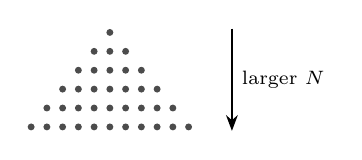
\begin{tikzpicture}
  \def\dx{0.2}\def\dy{0.24}
  \foreach \r in {1,...,6}{
    \pgfmathtruncatemacro\nr{2*\r-1}
    \foreach \k in {1,...,\nr}{
      \node[circle, fill=black!70, inner sep=0pt, minimum size=2.5pt] at ({(\k-(\nr+1)/2)*\dx}, {-(\r-1)*\dy}) {};
    }
  }
  \draw[-{Stealth}, semithick] (1.55,0.05) -- (1.55,-1.25) node[midway, right, font=\scriptsize]{larger $N$};
\end{tikzpicture}\\
{\scriptsize each row $=$ one population (units $=$ dots); down the rows, $N$ grows}
\end{center}
\begin{itemize} \vfill
\item Index by size $N$: estimator $\hat{\tau}_N$, ATE $\bar{\tau}_N$, group sizes $n_{1,N}, n_{0,N}$ \vfill
\item[] Subscript $N$ tracks the sequence; that lets us send $N \to \infty$ \vfill
\item Why care? Actual $N$ is finite, but the limit \mh{approximates} a large fixed $N$ \vfill
\end{itemize} \vfill
\end{frame}
%------------------------------------------------------------------------
\begin{frame}[t]{Two conditions for the variance to vanish}
\vfill
\begin{itemize} \vfill
\item Consistency needs $\Var[\hat{\tau}_N] \to 0$ as $N$ grows, where
\begin{equation*}
\Var[\hat{\tau}_N] = \frac{S^2_{\bm{y}(\bm{1}),N}}{n_{1,N}} + \frac{S^2_{\bm{y}(\bm{0}),N}}{n_{0,N}} - \frac{S^2_{\bm{\tau},N}}{N}
\end{equation*} \vfill
\item \mh{Treated share} converges to $p \in (0,1)$: both $n_{1,N}, n_{0,N}$ grow $\to \infty$ \vfill
\item[] If a group's share $\to 0$, group stays tiny and its term never shrinks \vfill
\item \mh{Bounded PO variance}: each $S^2_{\cdot, N}$ stays below a fixed ceiling \vfill
\item[] Else added units could be more and more extreme, growing the spread \vfill
\item Together: each term $=$ \mh{capped} numerator $/$ \mh{growing} denominator $\to 0$ \vfill
\end{itemize} \vfill
\end{frame}
%------------------------------------------------------------------------
\begin{frame}[t]{Vanishing variance gives consistency}
\vfill
\begin{itemize} \vfill
\item By \mh{Chebyshev Inequality}, \mh{variance} bounds distance from \mh{expected value} \vfill
\item[] For any $\epsilon > 0$,
\begin{equation*}
\Pr\left(\left\lvert \hat{\tau}_N - \E[\hat{\tau}_N] \right\rvert \geq \epsilon\right) \leq \frac{\Var[\hat{\tau}_N]}{\epsilon^2}
\end{equation*} \vfill
\item[] Smaller variance $\Rightarrow$ tighter bound $\Rightarrow$ $\hat{\tau}_N$ pinned near $\E[\hat{\tau}_N]$ \vfill
\item Unbiased, so $\E[\hat{\tau}_N] = \bar{\tau}_N$; and $\Var[\hat{\tau}_N] \to 0$ as $N$ grows, hence \vfill
\begin{equation*}
\Pr\left(\left\lvert \hat{\tau}_N - \bar{\tau}_N \right\rvert \geq \epsilon\right) \longrightarrow 0
\end{equation*} \vfill
\end{itemize} \vfill
\end{frame}
%------------------------------------------------------------------------
\begin{frame}[t]{What convergence in probability means}
\vfill
\begin{itemize} \vfill
\item Equivalently, for \emph{every} tolerance $\epsilon > 0$, \vfill
\begin{equation*}
\Pr\left(\left\lvert \hat{\tau}_N - \bar{\tau}_N \right\rvert < \epsilon\right) \to 1 \quad \text{as } N \to \infty
\end{equation*} \vfill
\item In words: fix any $\epsilon > 0$, however small \vfill
\begin{itemize} \vfill
\item For large enough $N$, $\hat{\tau}_N$ lands within $\epsilon$ of $\bar{\tau}_N$ with probability near $1$ \vfill
\end{itemize} \vfill
\item This is \mh{convergence in probability}: $\hat{\tau}_N - \bar{\tau}_N \overset{p}{\to} 0$ \vfill
\item The estimator \mh{concentrates} on its own population's ATE $\bar{\tau}_N$ \vfill
\end{itemize} \vfill
\end{frame}
%------------------------------------------------------------------------
\begin{frame}{Consistency in the village heads example}
\begin{itemize}
\item Stack copies of the $7$ villages; the distribution tightens on $\bar{\tau} = 5$:
\item[]
\begin{figure}[H]
\includegraphics[width=\linewidth]{figures/consistency_sim_plot.pdf}
\end{figure}
\item[] \footnotesize Estimator's distribution concentrates on $\bar{\tau} = 5$ (dashed) as $N$ grows. Exact for $N = 7, 14$; simulated ($10^5$ assignments) for $N = 28, 56$.
\end{itemize}
\end{frame}
%------------------------------------------------------------------------
\section{ACORN application}

\begin{frame}[t]{ACORN voter mobilization: the same logic}
\vfill
\begin{itemize} \vfill
\item Kansas City, 2003: ACORN \mh{door-to-door} GOTV \citep{arceneaux2005} \vfill
\item $N = 28$ precincts; CRA of $n_1 = 14$ canvassed, $n_0 = 14$ control \vfill
\item Outcome $y_i$: 2003 precinct \mh{turnout} proportion \vfill
\item Same machinery: estimand $\bar{\tau}$, estimator $\hat{\tau}\left(\bm{Z}, \bm{Y}\right)$, $\E[Z_i] = n_1/N$ \vfill
\item Mirrors Assignment 1, which uses these same precincts \vfill
\end{itemize} \vfill
\end{frame}
%------------------------------------------------------------------------
\begin{frame}[fragile]{ACORN in \texttt{R}: the estimate}
\begin{lstlisting}[style=Rstyle, basicstyle=\ttfamily\tiny, frame=single]
# ACORN GOTV experiment: 28 precincts, complete random assignment
acorn  <- read.csv("acorn03.csv")
z_obs  <- acorn$z           # 1 = canvassed (GOTV), 0 = control
y_obs  <- acorn$vote03      # observed 2003 turnout proportion
N  <- length(z_obs); n1 <- sum(z_obs); n0 <- N - n1   # 28, 14, 14

# Difference-in-Means estimator of the ATE: treated mean - control mean
diff_in_means <- function(z, y) mean(y[z == 1]) - mean(y[z == 0])
tau_hat <- diff_in_means(z = z_obs, y = y_obs)   # ~ 0.036 (about 3.6 points)
\end{lstlisting}
\begin{itemize} \vfill
\item \mh{Unbiased} for $\bar{\tau}$ by the identical argument \vfill
\item True $\Var\left[\hat{\tau}\right]$ needs \emph{both} POs per precinct \vfill
\item[] Conservative estimation tomorrow \vfill
\end{itemize}
\end{frame}
%------------------------------------------------------------------------
\begin{frame}[t]{Parallel to Assignment 1: the sharp null}
\small
\begin{itemize} \vfill
\item \mh{Sharp null of no effect}: $y_i(1) = y_i(0) = y_i$, so $\bm{y}$ \mh{fixed} \vfill
\item Assignment 1's statistic is the \mh{treated-group mean} $n_1^{-1}\bm{Z}^{\top}\bm{Y}$, estimating $\bar{y}$ \vfill
\item Over the assignment process (via $\E[Z_i] = n_1/N$): \vfill 
\begin{equation*}
\E\left[n_1^{-1}\bm{Z}^{\top}\bm{Y}\right] = \bar{y}, \quad \E\left[n_0^{-1}\left(\bm{1} - \bm{Z}\right)^{\top}\bm{Y}\right] = \bar{y}, \quad \E\left[\hat{\tau}\left(\bm{Z}, \bm{Y}\right)\right] = 0
\end{equation*} \vfill
\item Treated-mean variance $=$ usual sample-mean variance $\times$ an \mh{FPC} (Assignment 1): \vfill
\begin{equation*}
\Var\left[n_1^{-1}\bm{Z}^{\top}\bm{Y}\right] = \frac{S^2_{\bm{y}}}{n_1} \times \underbrace{\frac{n_0}{N}}_{\text{FPC}}
\end{equation*} \vfill
\item[] $S^2_{\bm{y}}/n_1$: the usual sample-mean variance, sampling \emph{with replacement} \vfill
\item[] FPC $n_0/N \le 1$ shrinks it \vfill
\item ACORN: $\bar{y} \approx 0.307$, $S^2_{\bm{y}} \approx 0.00435$; FPC $n_0/N = 1/2$ \emph{halves} $S^2_{\bm{y}}/n_1$ \vfill
\end{itemize} \vfill
\end{frame}
%------------------------------------------------------------------------
\begin{frame}[fragile]{ACORN in \texttt{R}: exact moments vs.\ simulation}
\begin{lstlisting}[style=Rstyle, basicstyle=\ttfamily\tiny, frame=single]
# Sharp null of no effect => y is FIXED; only the assignment is random.
# |Omega| = choose(28, 14) = 40,116,600 assignments: too many to enumerate,
# so compare EXACT design-based formulas with a Monte Carlo approximation.
ybar <- mean(y_obs)
Sy2  <- sum((y_obs - ybar)^2) / (N - 1)       # finite-population variance
E_treated_exact <- ybar                       # E[treated mean] = grand mean
Var_D_exact     <- Sy2 * (1/n1 + 1/n0)        # exact Var[diff-in-means]

set.seed(seed = 12345)                        # Monte Carlo over assignments
D <- replicate(n = 10^4, expr = diff_in_means(z = sample(x = z_obs), y = y_obs))
mean(D)   # ~ 0        : matches E[diff-in-means] = 0
var(D)    # ~ 0.00062  : matches Var_D_exact
\end{lstlisting}
\begin{itemize} \vfill
\item Simulation matches the exact design-based moments \vfill
\end{itemize}
\end{frame}
%------------------------------------------------------------------------
\section{Recap}

\begin{frame}[t]{Recap: estimating the average effect}
\vfill
\begin{itemize} \vfill
\item \mh{ATE} $\bar{\tau}$: a composite, average claim --- not a sharp one \vfill
\item \mh{Difference-in-means}: unbiased for $\bar{\tau}$ under random assignment \vfill
\item \mh{Variance} set by spread of potential outcomes and group sizes \vfill
\item \mh{Consistent}: unbiased $+$ variance $\to 0$ over a sequence of finite populations \vfill
\item All from the \mh{assignment mechanism} \vfill
\end{itemize} \vfill
\end{frame}
%------------------------------------------------------------------------
\begin{frame}[t]{Tomorrow}
\vfill
\begin{itemize} \vfill
\item \mh{Conservative} variance estimation (the unestimable $S^2_{\bm{\tau}}$ term) \vfill
\item \mh{Normal approximation} to the randomization distribution \vfill
\item \mh{$p$-values} and \mh{confidence intervals} for $\bar{\tau}$ \vfill
\item \mh{Covariance adjustment}: use covariates to reduce the estimator's variance \vfill
\end{itemize} \vfill
\end{frame}
%------------------------------------------------------------------------

\begin{frame}[allowframebreaks]
\frametitle{References}
\scriptsize
\bibliographystyle{chicago}
\bibliography{Master_Bibliography}
\end{frame}
%------------------------------------------------------------------------
\section{Appendix}

\begin{frame}[t]{Appendix: group-mean variances and the FPC}
\vfill
\begin{itemize} \vfill
\item Each group mean is a \mh{without-replacement} sample mean $\Rightarrow$ an \mh{FPC} \vfill
\item[] FPC $=$ share left to the other arm (intuition on the Assignment-1 slide):
\begin{equation*}
\Var[\bar{Y}_1] = \frac{S^2_{\bm{y}(\bm{1})}}{n_1}\underbrace{\frac{n_0}{N}}_{\text{FPC}}, \qquad
\Var[\bar{Y}_0] = \frac{S^2_{\bm{y}(\bm{0})}}{n_0}\underbrace{\frac{n_1}{N}}_{\text{FPC}}
\end{equation*}
\end{itemize}
\vfill
\end{frame}
%------------------------------------------------------------------------
\begin{frame}[t]{Appendix: expanding the FPC terms}
\vfill
\begin{itemize} \vfill
\item Write the FPC as $\tfrac{n_0}{N} = 1 - \tfrac{n_1}{N}$, then multiply out (control analogous): \vfill 
\begin{align*}
\Var[\bar{Y}_1] = \frac{S^2_{\bm{y}(\bm{1})}}{n_1}\left(1 - \tfrac{n_1}{N}\right)
&= \frac{S^2_{\bm{y}(\bm{1})}}{n_1} - \frac{S^2_{\bm{y}(\bm{1})}}{n_1}\cdot\frac{n_1}{N} \\
&= \frac{S^2_{\bm{y}(\bm{1})}}{n_1} - \frac{S^2_{\bm{y}(\bm{1})}}{N}
\end{align*} \vfill
\item[] Likewise $\Var[\bar{Y}_0] = \dfrac{S^2_{\bm{y}(\bm{0})}}{n_0} - \dfrac{S^2_{\bm{y}(\bm{0})}}{N}$ \vfill
\item These $-S^2/N$ pieces collect into Neyman's $-S^2_{\bm{\tau}}/N$ \vfill
\end{itemize} \vfill
\end{frame}
%------------------------------------------------------------------------
\begin{frame}[t]{Appendix: collecting into Neyman's variance}
\small
\begin{itemize} \vfill
\item \mh{Variance of a difference}: $\Var[\hat{\tau}] = \Var[\bar{Y}_1] + \Var[\bar{Y}_0] - 2\,\Cov[\bar{Y}_1, \bar{Y}_0]$ \vfill
\item Pieces: $\Var[\bar{Y}_{\cdot}]$ with FPC (above); $\Cov[\bar{Y}_1, \bar{Y}_0] = -S_{\bm{y}(\bm{0}),\bm{y}(\bm{1})}/N$ \vfill
\item Substitute ($-2\Cov = +2 S_{\bm{y}(\bm{0}),\bm{y}(\bm{1})}/N$): \vfill
\begin{align*}
\Var[\hat{\tau}\left(\bm{Z}, \bm{Y}\right)]
&= \frac{S^2_{\bm{y}(\bm{1})}}{n_1} - \frac{S^2_{\bm{y}(\bm{1})}}{N} + \frac{S^2_{\bm{y}(\bm{0})}}{n_0} - \frac{S^2_{\bm{y}(\bm{0})}}{N} + \frac{2 S_{\bm{y}(\bm{0}),\bm{y}(\bm{1})}}{N} \\
&= \frac{S^2_{\bm{y}(\bm{1})}}{n_1} + \frac{S^2_{\bm{y}(\bm{0})}}{n_0} - \frac{S^2_{\bm{y}(\bm{1})} + S^2_{\bm{y}(\bm{0})} - 2 S_{\bm{y}(\bm{0}),\bm{y}(\bm{1})}}{N}
\end{align*} \vfill
\item Numerator $= S^2_{\bm{\tau}}$ --- \mh{Neyman's variance}; $S^2_{\bm{\tau}}$ \emph{cannot} be estimated \vfill
\end{itemize} \vfill
\end{frame}
%------------------------------------------------------------------------
\begin{frame}[t]{Appendix: an equivalent variance form}
\vfill
\begin{itemize} \vfill
\item Neyman's \citeyearpar{neyman1923} original form, equivalent to the one in the main slides:
\begin{equation*}
\Var\left[\hat{\tau}\left(\bm{Z}, \bm{Y}\right)\right] = \frac{1}{N - 1}\left(\frac{n_1\, \sigma^2_{\bm{y}(\bm{0})}}{n_0} + \frac{n_0\, \sigma^2_{\bm{y}(\bm{1})}}{n_1} + 2\sigma_{\bm{y}(\bm{0}), \bm{y}(\bm{1})}\right)
\end{equation*}
where $\sigma^2$, $\sigma$ use the $\tfrac{1}{N}$ (population) convention \vfill
\item Village heads: $\sigma^2_{\bm{y}(\bm{0})} \approx 14.29$, $\sigma^2_{\bm{y}(\bm{1})} \approx 42.86$, $\sigma_{\bm{y}(\bm{0}), \bm{y}(\bm{1})} \approx 7.14$ \vfill
\item[] $\Rightarrow \Var\left[\hat{\tau}\left(\bm{Z}, \bm{Y}\right)\right] \approx 21.19$ \vfill
\end{itemize} \vfill
\end{frame}
%------------------------------------------------------------------------
\end{document}
